\subsection{Cartesian squares constructed by products, fibered products, and sums}

PROPOSITION 5. --- Let I be a set and, for every \(i \in I\) , let

\[
\begin{array}{c} \mathrm{X} _ {i} ^ {\prime} \xrightarrow {f _ {i} ^ {\prime}} \mathrm{X} _ {i} \\ \Big \downarrow p _ {i} ^ {\prime} \\ \mathrm{B} _ {i} ^ {\prime} \xrightarrow {f _ {i}} \mathrm{B} _ {i} \end{array}\tag{7}
\]

a cartesian square. The square

\[
\begin{array}{c} \prod_ {i \in \mathrm{I}} \mathrm{X} _ {i} ^ {\prime} \xrightarrow {f ^ {\prime}} \prod_ {i \in \mathrm{I}} \mathrm{X} _ {i} \\ \Biggl \downarrow^ {p ^ {\prime}} \qquad \qquad \qquad \qquad \Biggl \downarrow^ {p} \\ \prod_ {i \in \mathrm{I}} \mathrm{B} _ {i} ^ {\prime} \xrightarrow {f} \prod_ {i \in \mathrm{I}} \mathrm{B} _ {i} \end{array}\tag{ (7') }
\]

\((\text{where } f, f', p, p' \text{ are the extensions of the families } (f_i), (f'_i), (p_i), (p'_i) \text{ to products}) \text{ is Cartesian.}\)

Let Y be a topological space, and let \(u \colon \mathrm{Y} \to \prod_{i} \mathrm{B}_{i}'\) and \(v \colon \mathrm{Y} \to \prod_{i} \mathrm{X}_{i}\) be continuous maps such that \(f \circ u = p \circ v\) . For \(i \in \mathrm{I}\) , set \(u_{i} = \mathrm{pr}_{i} \circ u\) and \(v_{i} = \mathrm{pr}_{i} \circ v\) ; we have \(f_{i} \circ u_{i} = p_{i} \circ v_{i}\) and there exists a unique continuous map \(w_{i} \colon \mathrm{Y} \to \mathrm{X}_{i}'\) such that \(p_{i}' \circ w_{i} = u_{i}\) and \(f_{i}' \circ w_{i} = v_{i}\) . Then, the map \(w = (w_{i})\) is a continuous map from Y into \(\prod_{i} \mathrm{X}_{i}'\) such that \(p' \circ w = u\) and \(f' \circ w = v\) and it is the only one having these properties.

COROLLARY 1. --- Let X be a B-space, let p be its projection, and let F be a topological space. The square

\[
\begin{array}{c} \mathrm{X} \times \mathrm{F} \xrightarrow {\operatorname{pr} _ {1}} \mathrm{X} \\ \Biggl \downarrow p \times \mathrm{Id} _ {\mathrm{F}} \\ \mathrm{B} \times \mathrm{F} \xrightarrow {\operatorname{pr} _ {1}} \mathrm{B} \end{array}\tag{8}
\]

is Cartesian.

Let P be a topological space reduced to a point. Corollary 1 follows from Prop. 5 applied to the Cartesian squares

\[
\begin{array}{l} \mathrm{X} \xrightarrow {\mathrm{Id} _ {\mathrm{X}}} \mathrm{X} \\ \Big \downarrow_ {p} \qquad \Big \downarrow_ {p} \\ \mathrm{B} \xrightarrow {\mathrm{Id} _ {\mathrm{B}}} \mathrm{B} \end{array} \qquad \text {and} \qquad \begin{array}{l} \mathrm{F} \longrightarrow \mathrm{P} \\ \Big \downarrow_ {\mathrm{Id} _ {\mathrm{F}}} \qquad \Big \downarrow_ {\mathrm{Id} _ {\mathrm{P}}} \\ \mathrm{F} \longrightarrow \mathrm{P}. \end{array}
\]

Let B and B' be topological spaces, and let \(f: B' \to B\) be a continuous map. Let I be a set and, for every \(i \in I\) , let \(X_i\) be a B-space, \(X'_i\) be a B'-space, and \(f'_i: X'_i \to X_i\) be a continuous map such that the square

\[
\begin{array}{c} \mathrm{X} _ {i} ^ {\prime} \xrightarrow {f _ {i} ^ {\prime}} \mathrm{X} _ {i} \\ \Big \downarrow \\ \mathrm{B} ^ {\prime} \xrightarrow {f} \mathrm{B} \end{array}\tag{9}
\]

is commutative. There exists a unique continuous map

\[
f ^ {\prime} \colon \prod_ {i \in \mathrm{I}} \mathrm{X} _ {i} ^ {\prime} \to \prod_ {i \in \mathrm{I}} \mathrm{X} _ {i}
\]

such that \(pr_{i} \circ f' = f_{i}' \circ pr_{i}\) for all \(i \in I\) and such that the square

\[
\begin{array}{c} \prod_ {i \in I} X _ {i} ^ {\prime} \xrightarrow {f ^ {\prime}} \prod_ {i \in I} X _ {i} \\ \Big \downarrow \qquad \qquad \qquad \qquad \Big \downarrow \\ B ^ {\prime} \xrightarrow {f} B \end{array}\tag{ (9') }
\]

is commutative (this last condition following from the others if I ≠ ∅): it is the map deduced from the map

\[
f \times \prod_ {i \in \mathrm{I}} f _ {i} ^ {\prime} \colon \mathrm{B} ^ {\prime} \times \prod_ {i \in \mathrm{I}} \mathrm{X} _ {i} ^ {\prime} \to \mathrm{B} \times \prod_ {i \in \mathrm{I}} \mathrm{X} _ {i}
\]

by passing to subsets. With these notations:

COROLLARY 2. --- If the square (9) is Cartesian for every \(i \in I\) , then the square ( \(9'\) ) is Cartesian.

From prop. 5 one deduces a Cartesian square

\[
\begin{array}{c} \mathrm{B} ^ {\prime} \times \prod_ {i} \mathrm{X} _ {i} ^ {\prime} \xrightarrow {\operatorname{Id} _ {\mathrm{B}} \times \prod_ {i} f _ {i} ^ {\prime}} \mathrm{B} \times \prod_ {i} \mathrm{X} _ {i} \\ \Biggl \downarrow \\ \mathrm{B} ^ {\prime} \times (\mathrm{B} ^ {\prime}) ^ {\mathrm{I}} \xrightarrow {f \times \prod_ {i} f} \mathrm{B} \times \mathrm{B} ^ {\mathrm{I}}  . \end{array}
\]

Denote by \(\Delta_{\mathrm{B}^{\prime}}\) and \(\Delta_{\mathrm{B}}\) the diagonals of \(\mathrm{B}^{\prime}\times (\mathrm{B}^{\prime})^{\mathrm{I}}\) and \(\mathrm{B}\times \mathrm{B}^{\mathrm{I}}\) . The diagram

\[
\begin{array}{c} \prod_ {i \in \mathrm{I}} X _ {i} ^ {\prime} \xrightarrow {f ^ {\prime}} \prod_ {i \in \mathrm{I}} X _ {i} \\ \Big \downarrow \qquad \qquad \qquad \Big \downarrow \\ \Delta_ {\mathrm{B} ^ {\prime}} \xrightarrow {} \Delta_ {\mathrm{B}} \end{array}
\]

deduced from the preceding one by passing to subspaces is Cartesian (I, p. 9, prop. 4). It is identified with diagram (9').

Example 1. --- Let

\[
\begin{array}{c} \mathrm {X^ {\prime}} \xrightarrow {f ^ {\prime}} \mathrm{X} \\ \Big \downarrow_ {p ^ {\prime}} \\ \mathrm {B^ {\prime}} \xrightarrow {f} \mathrm{B} \end{array}
\]

a Cartesian square. Then Corollary 2 provides a Cartesian square

\[
\begin{array}{c} \mathrm {X^ {\prime} \times_ {B^ {\prime}} X^ {\prime}} \xrightarrow {\varphi} \mathrm {X\times_ {B} X} \\ \Big \downarrow \\ \mathrm {B^ {\prime} \xrightarrow {f} B}. \end{array}
\]

We have the relation \(\overline{\varphi}^{1}(\Delta_{\mathrm{X}}) = \Delta_{\mathrm{X}^{\prime}}\) . Indeed, by Proposition 2 of I, p. 8, it suffices to consider the case where \(\mathrm{X}' = \mathrm{B}' \times_{\mathrm{B}} \mathrm{X}\) . Let then \(((b,x),(b,x'))\) be an element of \(X^{\prime} \times_{B^{\prime}} X^{\prime}\) with \(b \in B^{\prime}\) and \(x, x^{\prime} \in X\) . This element belongs to \(\overline{\varphi}^{1}(\Delta_{\mathrm{X}})\) if and only if \(x = x^{\prime}\) .

PROPOSITION 6. --- Let I be a set and, for every \(i \in I\) , let

\[
\begin{array}{c} \mathrm{X} _ {i} ^ {\prime} \xrightarrow {f _ {i} ^ {\prime}} \mathrm{X} \\ \Biggl \downarrow p _ {i} ^ {\prime} \\ \mathrm{B} _ {i} ^ {\prime} \xrightarrow {f _ {i}} \mathrm{B} \end{array}\tag{10}
\]

a Cartesian square. Let X' and B' be the sum spaces of the families \((X'_i)\) and \((B'_i)\), respectively. Let f: B' → B, f': X' → X, and p': X' → B' be the maps induced from the families \((f_i)\), \((f'_i)\), and \((p'_i)\), respectively. The square

\((10')\)

\pandocbounded{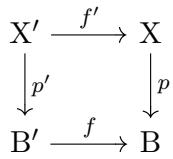
\includegraphics[keepaspectratio]{images/part001_48571453.jpg}}

is Cartesian.

The maps \(f\) , \(f'\) , and \(p'\) are continuous. The commutativity of the square \((10')\) follows from its definition. Let \(h_i\) denote the canonical homeomorphism from \(\mathrm{X}_i'\) onto \(\mathrm{B}_i' \times_{\mathrm{B}} \mathrm{X}\) (I, p. 8, Proposition 2) and let \(h: \mathrm{X}' \to \mathrm{B}' \times_{\mathrm{B}} \mathrm{X}\) be the canonical map (loc. cit.). We have \(h = h'' \circ h'\) , where \(h': \mathrm{X}' \to \coprod (\mathrm{B}_i' \times_{\mathrm{B}} \mathrm{X})\) is the homeomorphism induced by the \(h_i\) and \(h'': \coprod (\mathrm{B}_i' \times_{\mathrm{B}} \mathrm{X}) \to (\coprod \mathrm{B}_i') \times_{\mathrm{B}} \mathrm{X}\) is the one defined in Example 5 of I, p. 4. We conclude by Proposition 2 of I, p. 8.

Example 2. --- Let \((X,p)\) be a B-space and let \((\mathrm{A}_{k})_{k\in\mathrm{K}}\) be a family of subspaces of B. Let A be the sum space of the family \((\mathrm{A}_{k})_{k\in\mathrm{K}}\) and let Y be the sum space of the family \((\overline{p}^{1}(\mathrm{A}_{k}))_{k\in\mathrm{K}}\) ; let us denote by \(i: A \to B\) , \(j: Y \to X\) , and \(p': Y \to A\) the maps induced by the canonical injections of \(A_{k}\) into B, the canonical injections of \(\overline{p}^{1}(\mathrm{A}_{k})\) into X, and the maps \(p_{\mathrm{A}_{k}}: \overline{p}^{1}(\mathrm{A}_{k}) \to \mathrm{A}_{k}\) , for \(k \in K\) . The square

\[
\begin{array}{c} \mathrm{Y} \xrightarrow {j} \mathrm{X} \\ \Biggl \downarrow p ^ {\prime} \\ \mathrm{A} \xrightarrow {i} \mathrm{B} \end{array}\tag{11}
\]

is Cartesian; this follows from the example in I, p. 10 and from Prop. 6.

